\documentclass[11pt,a4paper]{article}

% --- Packages ---
\usepackage[utf8]{inputenc}
\usepackage[english]{babel}
\usepackage{amsmath,amssymb}
\usepackage{graphicx}
\usepackage{booktabs}        % Profesyonel tablolar için
\usepackage{caption}
\usepackage{subcaption}
\usepackage[margin=2.5cm]{geometry}
\usepackage{hyperref}
\usepackage{xcolor}
\usepackage{listings}
\usepackage{float}           % H placement için
\usepackage{titling}
\usepackage{enumitem}
\usepackage{multirow}
\usepackage{array}

% --- Hyperlink colors ---
\hypersetup{
    colorlinks=true,
    linkcolor=blue!50!black,
    citecolor=blue!50!black,
    urlcolor=blue!50!black,
}

% --- Code listing style ---
\lstset{
    basicstyle=\ttfamily\small,
    breaklines=true,
    frame=single,
    backgroundcolor=\color{gray!10},
    showstringspaces=false,
}

% --- Title ---
\title{
    \vspace{-2cm}
    \large CENG 467 -- Natural Language Understanding and Generation \\
    \Large \textbf{Take-Home Midterm Report}
}
\author{
    İrem Cesur \\
    Student ID: 310201051 \\
    \href{https://github.com/iremcesur/CENG467_Midterm_310201051}{https://github.com/iremcesur/CENG467\_Midterm\_310201051}
}
\date{April 2026}

\begin{document}

\maketitle

\begin{abstract}
\noindent
This report presents a comprehensive empirical study across five core NLP tasks: text classification, named entity recognition, abstractive and extractive summarization, machine translation, and language modeling. For each task, multiple representational paradigms are compared under controlled experimental conditions, with consistent dataset splits, preprocessing pipelines, and evaluation protocols. We report quantitative metrics, qualitative error analyses, and discuss trade-offs between classical, recurrent, and transformer-based approaches. All experiments are fully reproducible via a fixed random seed (42); code and configurations are publicly available.
\end{abstract}

\tableofcontents
\newpage

% =========================================================
\section{Introduction}
\label{sec:intro}

This report addresses the five questions of the CENG 467 take-home midterm. Each section follows a uniform structure: problem formulation, dataset description, methodological decisions, experimental setup, results, and discussion. The objective is not solely to optimize predictive performance, but to characterize model behavior, expose failure modes, and analyze trade-offs across representation paradigms.

All experiments use a single random seed ($\texttt{SEED}=42$) applied to Python, NumPy, and PyTorch where applicable. Training, validation, and test splits are fixed in advance and shared across models within each task. The test set is consulted exactly once per model for final evaluation. Hyperparameters are tuned only on the validation set.

% =========================================================
\section{Question 1: Representation Learning in Text Classification}
\label{sec:q1}

\subsection{Problem Formulation}

Sentiment classification on movie reviews is framed as a binary text classification task: given a review document $x$, predict $y \in \{\text{negative}, \text{positive}\}$. The objective is to compare three paradigms of textual representation:
\begin{itemize}[noitemsep]
    \item \textbf{Sparse:} TF-IDF features with a linear classifier.
    \item \textbf{Dense (static):} pre-trained word embeddings combined with a recurrent neural model.
    \item \textbf{Contextual:} a transformer-based model with subword tokenization and contextualized representations.
\end{itemize}
All three models share an identical train/validation/test partition, ensuring that observed performance differences are attributable to representation choice rather than data variability.

\subsection{Dataset}

We use the \textbf{IMDb Large Movie Review Dataset} \cite{maas2011imdb}, accessed via the HuggingFace \texttt{datasets} library. The corpus contains 50{,}000 polarized reviews (25{,}000 train, 25{,}000 test) labeled as positive or negative, with an exactly balanced class distribution. Reviews are unstructured English text with substantial length variation: many exceed 500 tokens, exposing models to a long-context regime.

\paragraph{Subsetting.} Due to compute constraints on free-tier Google Colab (T4 GPU, limited session duration), we use a stratified subset:
\begin{itemize}[noitemsep]
    \item \textbf{Train:} 5{,}000 reviews (2{,}493 negative / 2{,}507 positive)
    \item \textbf{Validation:} 1{,}000 reviews (499 / 501)
    \item \textbf{Test:} 2{,}000 reviews (1{,}040 / 960)
\end{itemize}
The validation split is carved from the original training partition via stratified sampling; the test split is drawn from the original test partition with random seeding. All three models in this section use this identical split. We acknowledge that smaller training sets may underestimate the upper-bound performance of transformer-based models, which typically benefit more from data scale; this is itself an interesting observation, addressed in Section~\ref{sec:q1-discussion}.

\subsection{Preprocessing and Tokenization}

We compare two tokenization strategies:
\begin{enumerate}[noitemsep]
    \item \textbf{Word-level tokenization} with optional lowercasing and English stopword removal (NLTK list, 198 tokens). Used by the TF-IDF model.
    \item \textbf{Subword (WordPiece) tokenization} via the pre-trained DistilBERT tokenizer. Used by the transformer.
\end{enumerate}
The BiLSTM uses a custom whitespace-based tokenizer with a 30{,}000-word vocabulary built from the training set, mapping out-of-vocabulary tokens to a dedicated \texttt{<unk>} symbol.

To analyze the effect of preprocessing decisions, we conduct an ablation study (Section~\ref{sec:q1-tfidf}) over two binary axes -- \emph{stopword removal} and \emph{n-gram range} -- on the TF-IDF model. Truncation effects are quantified for the transformer in Section~\ref{sec:q1-bert}.

\subsection{Models}

\subsubsection{TF-IDF + Logistic Regression}
\label{sec:q1-tfidf}

\paragraph{Method.} Documents are vectorized with \texttt{TfidfVectorizer} (scikit-learn) using sublinear term-frequency scaling. A Logistic Regression classifier ($C=1.0$, \texttt{liblinear} solver) is trained on the resulting sparse representation.

\paragraph{Ablation.} We evaluate four configurations on the validation set, varying stopword removal and n-gram range while keeping all other hyperparameters fixed (Table~\ref{tab:tfidf-ablation}).

\begin{table}[H]
\centering
\caption{TF-IDF ablation study on the validation set. All configurations use lowercase normalization, sublinear TF, $\texttt{max\_features}=20{,}000$, and identical Logistic Regression hyperparameters.}
\label{tab:tfidf-ablation}
\begin{tabular}{lccc}
\toprule
\textbf{Configuration} & \textbf{Val Accuracy} & \textbf{Val Macro-F1} & \textbf{Time (s)} \\
\midrule
1. Baseline (unigram)              & 0.8570 & 0.8570 & 5.9 \\
2. + Stopword removal              & 0.8560 & 0.8559 & 3.2 \\
3. + Bigrams (uni+bi)              & 0.8640 & 0.8640 & 12.1 \\
4. \textbf{Bigrams + Stopword removal} & \textbf{0.8690} & \textbf{0.8689} & 9.6 \\
\bottomrule
\end{tabular}
\end{table}

\paragraph{Observations.} Three findings are noteworthy:
\begin{enumerate}[noitemsep]
    \item \textbf{Stopword removal alone slightly hurts performance} ($-0.001$ Macro-F1). This is consistent with sentiment-analysis intuition: tokens such as \emph{not}, \emph{very}, \emph{no} carry significant polarity information that the generic English stopword list discards.
    \item \textbf{Adding bigrams yields a meaningful gain} ($+0.007$). Bigrams capture two-word patterns -- \emph{not good}, \emph{really enjoyed}, \emph{very bad} -- that unigram representations cannot distinguish from their constituent words taken in isolation.
    \item \textbf{Bigrams and stopword removal interact positively} when combined ($+0.012$ over baseline). Once bigrams capture phrasal sentiment, removing high-frequency stopwords reduces noise without sacrificing polarity-bearing context.
\end{enumerate}

\paragraph{Final test results.} Configuration~4 was selected based on validation performance and evaluated once on the held-out test set (Table~\ref{tab:tfidf-test}, Figure~\ref{fig:tfidf-cm}).

\begin{table}[H]
\centering
\caption{TF-IDF + Logistic Regression -- final test set performance.}
\label{tab:tfidf-test}
\begin{tabular}{lcc}
\toprule
\textbf{Class} & \textbf{Precision} & \textbf{Recall} \\
\midrule
Negative & 0.8934 & 0.8462 \\
Positive & 0.8424 & 0.8906 \\
\midrule
\textbf{Macro avg} & \textbf{0.8679} & \textbf{0.8684} \\
\bottomrule
\end{tabular}
\quad
\begin{tabular}{lc}
\toprule
\textbf{Metric} & \textbf{Value} \\
\midrule
Test Accuracy   & 0.8675 \\
Test Macro-F1   & 0.8675 \\
Misclassified   & 265 / 2{,}000 (13.2\%) \\
\bottomrule
\end{tabular}
\end{table}

\begin{figure}[H]
\centering
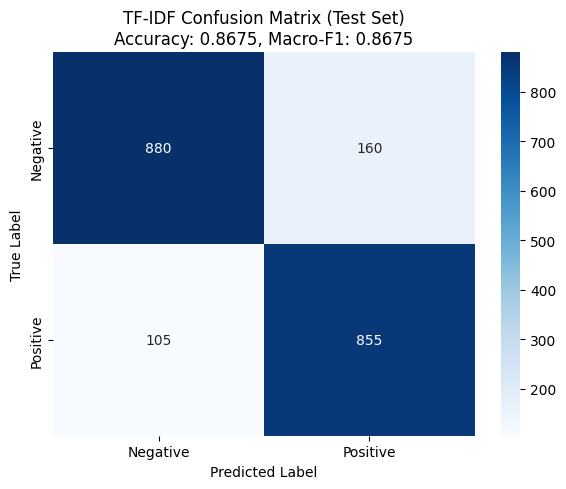
\includegraphics[width=0.55\textwidth]{figures/tf-idf.png}
\caption{Confusion matrix on the test set. The classifier exhibits asymmetric error patterns: false positives (160) outnumber false negatives (105), indicating that mixed-sentiment negative reviews are harder to identify than mixed-sentiment positive ones.}
\label{fig:tfidf-cm}
\end{figure}

The validation-to-test gap is small (0.8689 $\rightarrow$ 0.8675 Macro-F1), suggesting that the model generalizes well within this evaluation regime and is not overfitting to validation idiosyncrasies.

\subsubsection{BiLSTM with GloVe Embeddings}
\label{sec:q1-bilstm}
\paragraph{Method.} The BiLSTM classifier consists of (i) a frozen embedding layer initialized with pre-trained GloVe 6B 100-dimensional vectors~\cite{pennington2014glove}, (ii) a single-layer bidirectional LSTM with 128 hidden units, (iii) a masked mean-pooling layer that averages BiLSTM outputs over non-padding positions, and (iv) a linear classifier with sigmoid output. Dropout (0.5) is applied to the pooled representation. Sequences are tokenized with a custom whitespace tokenizer (after lowercasing and HTML-tag removal) and truncated to 256 tokens.

\paragraph{Vocabulary and embeddings.} A vocabulary of 30{,}000 most frequent training tokens is built; out-of-vocabulary tokens map to a dedicated $\langle\texttt{unk}\rangle$ symbol. The embedding matrix is constructed by looking up each vocabulary entry in GloVe; \textbf{88.2\% of vocabulary tokens are covered} by GloVe, with the remaining 11.8\% (mostly proper nouns, misspellings, and tokenizer artifacts such as \emph{don't} $\rightarrow$ \emph{don}, \emph{t}) initialized to zero vectors. Since the embedding layer is frozen, these out-of-vocabulary tokens contribute no learned signal.

\paragraph{Training setup.} The model has 3.24M total parameters, of which 235{,}777 are trainable (the embedding layer accounts for the rest and is frozen). We train with Adam (learning rate $10^{-3}$, batch size 64), binary cross-entropy loss, and gradient clipping at $\ell_2$ norm 5. Training is capped at 15 epochs with early stopping (patience 4) on validation Macro-F1. The best model checkpoint is restored after training.

\paragraph{Training dynamics.} Training converges over approximately 13 epochs (Figure~\ref{fig:bilstm-curves}). Train accuracy rises monotonically from 0.61 to 0.89, while validation Macro-F1 plateaus around 0.85 and exhibits noisier, non-monotonic behavior characteristic of small-data regimes. The validation loss spike at epoch 9 reflects sensitivity to mini-batch composition rather than systematic degradation. The best epoch (13) is selected based on Macro-F1; epochs beyond this point show widening train-validation gap, indicative of mild overfitting.

\begin{figure}[H]
\centering
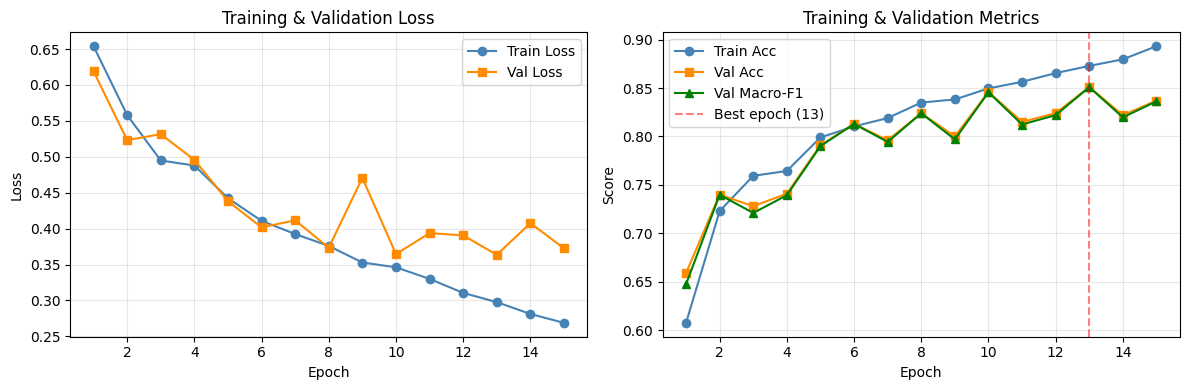
\includegraphics[width=\textwidth]{figures/bilstm_training_curves.png}
\caption{BiLSTM training curves. Left: training and validation loss. Right: training accuracy, validation accuracy, and validation Macro-F1; the dashed red line marks the best epoch (13) selected for final evaluation.}
\label{fig:bilstm-curves}
\end{figure}

\paragraph{Final test results.} The restored best-epoch model is evaluated once on the test set (Table~\ref{tab:bilstm-test}, Figure~\ref{fig:bilstm-cm}).

\begin{table}[H]
\centering
\caption{BiLSTM + GloVe -- final test set performance.}
\label{tab:bilstm-test}
\begin{tabular}{lcc}
\toprule
\textbf{Class} & \textbf{Precision} & \textbf{Recall} \\
\midrule
Negative & 0.8507 & 0.8712 \\
Positive & 0.8567 & 0.8344 \\
\midrule
\textbf{Macro avg} & \textbf{0.8537} & \textbf{0.8528} \\
\bottomrule
\end{tabular}
\quad
\begin{tabular}{lc}
\toprule
\textbf{Metric} & \textbf{Value} \\
\midrule
Test Accuracy & 0.8535 \\
Test Macro-F1 & 0.8531 \\
Misclassified & 293 / 2{,}000 (14.7\%) \\
\bottomrule
\end{tabular}
\end{table}

\begin{figure}[H]
\centering
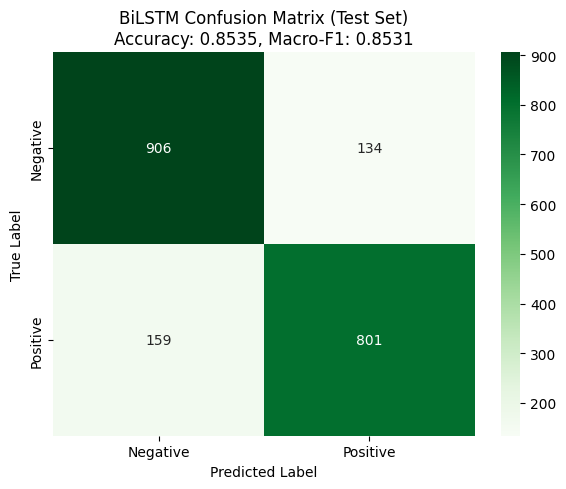
\includegraphics[width=0.55\textwidth]{figures/bilstm_confusion_matrix.png}
\caption{BiLSTM confusion matrix on the test set. Compared to TF-IDF (Figure~\ref{fig:tfidf-cm}), the BiLSTM exhibits an inverted error asymmetry: false negatives (159) outnumber false positives (134), suggesting a more conservative bias toward predicting the negative class.}
\label{fig:bilstm-cm}
\end{figure}

\paragraph{Underperformance analysis.} The BiLSTM achieves test Macro-F1 of 0.8531, slightly below the TF-IDF baseline (0.8675). This counterintuitive result -- a sequence-aware neural model trailing a bag-of-words classifier -- is informative and we attribute it to four interacting factors:
\begin{enumerate}[noitemsep]
    \item \textbf{Limited training data.} With 5{,}000 training examples, neural models are constrained; published BiLSTM-on-IMDb results typically use 25{,}000+ examples and approach 88--90\% accuracy. Our subset is too small to fully exploit the additional capacity offered by sequence modeling.
    \item \textbf{Frozen embeddings with imperfect coverage.} Roughly 12\% of in-vocabulary tokens lack GloVe vectors and contribute no signal. Fine-tuning the embedding layer (left as future work) could substantially improve this.
    \item \textbf{Sequence truncation.} Reviews are truncated to 256 tokens, while TF-IDF observes the full document. For long reviews where sentiment is concentrated in later paragraphs, the BiLSTM is at a structural disadvantage.
    \item \textbf{Strong baseline.} Bigram TF-IDF already captures most polarity-bearing phrasal patterns (\emph{not good}, \emph{very enjoyable}); the additional contextual modeling offered by a recurrent network yields diminishing returns at this scale.
\end{enumerate}
The error-mode analysis (Figure~\ref{fig:bilstm-cm}) reveals an additional finding: the BiLSTM's errors are \emph{qualitatively different} from those of TF-IDF (negative-leaning vs.\ positive-leaning bias). This complementarity will be revisited in the cross-model error analysis (Section~\ref{sec:q1-discussion}).


\textit{[To be completed in the next session.]}

\subsubsection{DistilBERT}
\label{sec:q1-bert}
\paragraph{Method.} We fine-tune the pre-trained \texttt{distilbert-base-uncased} model~\cite{sanh2019distilbert} on our IMDb subset using the HuggingFace \texttt{transformers} library. DistilBERT is a 6-layer transformer (66M parameters) distilled from BERT-base, retaining 97\% of BERT's language-understanding capability while being 60\% faster. The pre-trained model uses WordPiece subword tokenization with a 30{,}522-token vocabulary -- crucially eliminating out-of-vocabulary issues that affected the BiLSTM. A linear classification head is attached to the \texttt{[CLS]} token's final hidden state.

\paragraph{Tokenization and truncation.} Reviews are tokenized with the DistilBERT tokenizer and truncated to 256 tokens, identical to the BiLSTM setup, ensuring all three models observe the same input window for direct comparability. Dynamic padding (per batch) is applied via a data collator to minimize wasted computation.

\paragraph{Training setup.} We perform full fine-tuning -- all 67M parameters are updated. Hyperparameters follow standard BERT fine-tuning practice: AdamW optimizer with learning rate $2 \times 10^{-5}$, weight decay 0.01, linear warmup over the first 94 steps (10\% of total), and batch size 16. We train for 3 epochs (sufficient for convergence on this dataset size, per published BERT/IMDb literature), with mixed-precision (fp16) training for $\sim$2$\times$ speedup on the T4 GPU. Early stopping (patience 2) on validation Macro-F1 is configured but not triggered. The best checkpoint by validation Macro-F1 is restored after training. Total training time: 137 seconds (2.3 minutes).

\paragraph{Training dynamics.} The model converges rapidly (Figure~\ref{fig:bert-curves}). Validation Macro-F1 climbs from 0.8592 (epoch 1) to 0.8879 (epoch 2) to 0.8970 (epoch 3). Training loss decreases monotonically (0.294 $\rightarrow$ 0.110), but validation loss exhibits a non-monotonic pattern: 0.322 $\rightarrow$ 0.309 $\rightarrow$ 0.346. This characteristic behavior -- decreasing accuracy-aligned metrics combined with rising cross-entropy loss -- indicates emerging \emph{overconfidence}: the model becomes increasingly certain on confident predictions while incorrectly-predicted examples receive sharper, more wrongly-confident probabilities. Since our selection criterion is Macro-F1 (not loss), the epoch-3 model is correctly retained.

\begin{figure}[H]
\centering
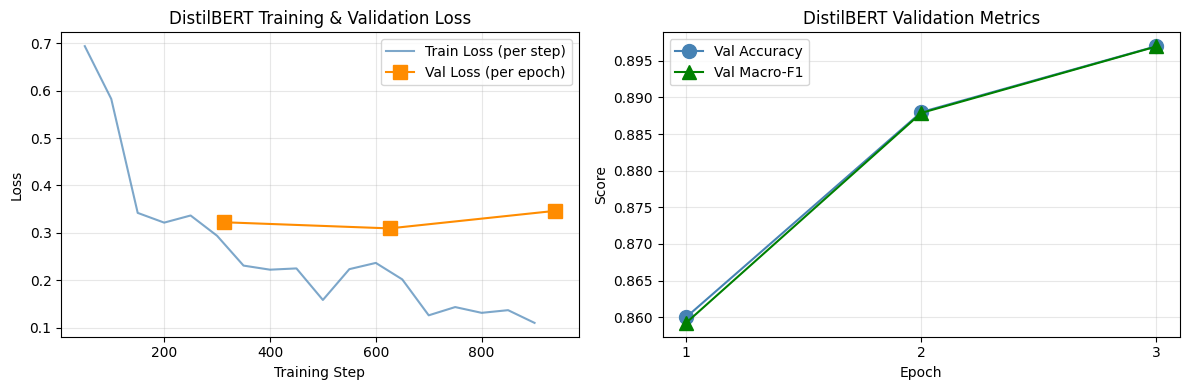
\includegraphics[width=\textwidth]{figures/distilbert_training_curves.png}
\caption{DistilBERT training curves. Left: per-step training loss and per-epoch validation loss; the divergence in the final epoch reflects increasing model confidence rather than degraded accuracy. Right: validation accuracy and Macro-F1 rise monotonically across all three epochs.}
\label{fig:bert-curves}
\end{figure}

\paragraph{Final test results.} The best-checkpoint model is evaluated once on the test set (Table~\ref{tab:bert-test}, Figure~\ref{fig:bert-cm}).

\begin{table}[H]
\centering
\caption{DistilBERT -- final test set performance.}
\label{tab:bert-test}
\begin{tabular}{lcc}
\toprule
\textbf{Class} & \textbf{Precision} & \textbf{Recall} \\
\midrule
Negative & 0.9036 & 0.9106 \\
Positive & 0.9023 & 0.8948 \\
\midrule
\textbf{Macro avg} & \textbf{0.9030} & \textbf{0.9027} \\
\bottomrule
\end{tabular}
\quad
\begin{tabular}{lc}
\toprule
\textbf{Metric} & \textbf{Value} \\
\midrule
Test Accuracy & 0.9030 \\
Test Macro-F1 & 0.9028 \\
Misclassified & 194 / 2{,}000 (9.7\%) \\
\bottomrule
\end{tabular}
\end{table}

\begin{figure}[H]
\centering
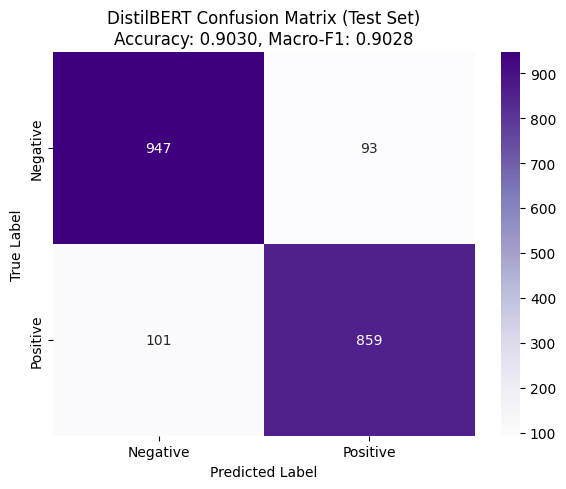
\includegraphics[width=0.55\textwidth]{figures/distilbert_confusion_matrix.png}
\caption{DistilBERT confusion matrix on the test set. Errors are nearly balanced between false positives (93) and false negatives (101), in contrast to the asymmetric biases observed for TF-IDF (positive-leaning) and BiLSTM (negative-leaning).}
\label{fig:bert-cm}
\end{figure}

DistilBERT outperforms both the TF-IDF baseline ($+3.5$ percentage points Macro-F1) and the BiLSTM ($+5.0$ percentage points), reducing the misclassification rate from 13.2\% (TF-IDF) and 14.7\% (BiLSTM) to 9.7\%. The validation-to-test gap is small (0.8970 $\rightarrow$ 0.9028, in fact a slight improvement on test), suggesting robust generalization. The per-class precision and recall are all within 0.01 of one another, indicating that the model has not learned a class-prior bias -- a meaningful advantage over the previous two models.

\subsection{Discussion}
\label{sec:q1-discussion}

\subsubsection{Consolidated Results}

Table~\ref{tab:q1-summary} consolidates the test-set performance of all three models alongside their parameter counts and training times. DistilBERT achieves the strongest performance on every metric, while incurring the highest compute cost; TF-IDF emerges as a remarkably competitive baseline at a fraction of the cost.

\begin{table}[H]
\centering
\caption{Question 1 -- consolidated test-set results across all three representation paradigms.}
\label{tab:q1-summary}
\begin{tabular}{lccccc}
\toprule
\textbf{Model} & \textbf{Test Acc} & \textbf{Test F1} & \textbf{Trainable Params} & \textbf{Train Time} & \textbf{Misclass.\ rate} \\
\midrule
TF-IDF + LogReg     & 0.8675 & 0.8675 & $\sim$20K  & 9.6 s   & 13.2\% \\
BiLSTM + GloVe      & 0.8535 & 0.8531 & 235{,}777  & 57 s    & 14.7\% \\
DistilBERT (FT)     & \textbf{0.9030} & \textbf{0.9028} & 66{,}955{,}010 & 137 s   & \textbf{9.7}\% \\
\bottomrule
\end{tabular}
\end{table}

\subsubsection{Cross-Model Error Analysis}

To characterize qualitative differences between models, we cross-tabulate per-example correctness across the 2{,}000 test predictions (Table~\ref{tab:cross-error}). Three findings stand out:

\begin{table}[H]
\centering
\caption{Cross-model error patterns on the test set.}
\label{tab:cross-error}
\begin{tabular}{lcc}
\toprule
\textbf{Pattern} & \textbf{Count} & \textbf{Share} \\
\midrule
All three models correct          & 1{,}513 & 75.6\% \\
All three models incorrect        & 71      & 3.5\% \\
Only DistilBERT correct           & 55      & 2.8\% \\
Only DistilBERT incorrect         & 55      & 2.8\% \\
\bottomrule
\end{tabular}
\end{table}

First, the majority of test examples (75.6\%) are easy in the sense that all three classifiers agree on the correct label; performance differences therefore arise on the remaining $\sim$25\% of harder examples. Second, 3.5\% of examples (71) defeat all three models simultaneously -- these are inherently ambiguous. Third, the symmetric counts of "Only BERT correct" (55) and "Only BERT incorrect" (55) are misleading on their own: while the net contribution looks neutral, the qualitative \emph{kinds} of examples in each group differ markedly, as the case studies below illustrate.

\paragraph{Case studies.} We hand-picked five representative misclassified examples spanning the three error categories. Each is shown with the true label, all three model predictions, and the predicted positive-class probability.

\begin{enumerate}[leftmargin=*]
    \item \textbf{Plot-summary trap (all three wrong, true=Negative).} The review of \emph{Ernest Saves Christmas} opens with a paragraph-long synopsis (``\ldots Ernest has to find a successor to Santa Claus\ldots'') laden with positive vocabulary (Christmas, special, saves). All three models predict Positive with high confidence (BERT: 0.996). The actual critique appears later in the review, beyond the 256-token truncation window for the BiLSTM and BERT, and is diluted by surface positives in the TF-IDF representation. \emph{Lesson:} truncation interacts adversely with reviews that buried sentiment at the end.

    \item \textbf{Sarcasm/snark (all three wrong, true=Negative).} The review of \emph{The Adventures of Sebastian Cole} uses ironic phrasing such as ``fancies himself becoming a writer\ldots given he actually puts effort into it.'' The literal vocabulary is neutral-to-positive; the negative sentiment is encoded in the implicature, not the lexicon. All three models predict Positive (BERT: 0.995). \emph{Lesson:} sarcasm detection remains an open problem; even contextual representations trained on web text struggle when irony is signaled by tone rather than explicit cues.

    \item \textbf{Concession structure (only BERT correct, true=Positive).} The review of an \emph{Angel}-fan film contains both positive markers (``sexy and original'', ``quite entertaining'') and qualifications (``feels a little inadequate''). TF-IDF and BiLSTM down-vote it (probabilities 0.474 and 0.373); DistilBERT correctly classifies it Positive (0.995). \emph{Lesson:} bag-of-words and frozen-embedding models overweight individual negative tokens, while contextual models can integrate them as minor concessions within a globally positive judgment.

    \item \textbf{``Despite\ldots but good enough'' (only BERT correct, true=Positive).} The \emph{Inki and the Minah Bird} review is a textbook \emph{concession-then-affirmation} structure: ``Despite looking dated\ldots'', ``isn't extraordinary, but good enough\ldots'', resolving in ``enjoyable and charming''. Both TF-IDF (0.477) and BiLSTM (0.329) are misled by the negation tokens; DistilBERT recovers the affirming conclusion (0.995). \emph{Lesson:} concessive constructions are a clear win for contextual representations -- they require composing meaning across multiple clauses rather than counting polarity-bearing words.

    \item \textbf{Front-loaded contrarian framing (only BERT wrong, true=Negative).} The review of a Dario Argento film opens with an ostensible defense (``called a lot of bad things by non-fans. And is deserving of absolutely none of the backlash\ldots''). DistilBERT reads this opening as positive (0.995) and locks onto it. TF-IDF and BiLSTM, being more local in their attention, weight the strong negative tokens (\emph{bad}, \emph{backlash}, \emph{absolutely none}) and -- by a different reasoning path -- arrive at the correct label. \emph{Lesson:} BERT's deeper composition can be a liability when an early misleading clause anchors interpretation. Bag-of-words models, lacking long-range composition, are sometimes \emph{accidentally robust} to such framing effects.
\end{enumerate}

\subsubsection{Representation Paradigm Trade-offs}

The empirical evidence supports a nuanced rather than monotonic ordering of representation paradigms.

\paragraph{Sparse representations (TF-IDF) are a strong, interpretable, and cheap baseline.} On a 5{,}000-document training set, bigram TF-IDF with logistic regression reaches 86.75\% accuracy in under 10 seconds. The model is fully introspectable -- coefficients map directly to (n-)grams -- and exhibits predictable failure modes (sarcasm, mixed sentiment). Its performance ceiling reflects the inherent limit of order-insensitive features, which our error analysis localizes specifically to concessive and ironic constructions.

\paragraph{Static dense representations (BiLSTM + frozen GloVe) underperform in this regime.} Despite being a sequence model, the BiLSTM trails TF-IDF by 1.4 percentage points. Section~\ref{sec:q1-bilstm} attributed this to four factors -- limited training data, embedding coverage gaps, sequence truncation, and a strong baseline -- which compound to leave the model unable to convert its theoretical advantage in word-order sensitivity into measurable gains. We expect this gap to close or invert with (i) larger training sets ($\geq$25k examples), (ii) fine-tuned (rather than frozen) embeddings, or (iii) deeper recurrent stacks.

\paragraph{Contextual representations (DistilBERT) deliver clear gains, but at non-trivial cost.} DistilBERT exceeds TF-IDF by 3.5 points and BiLSTM by 5.0 points on Macro-F1. The gain is concentrated on examples requiring multi-clause integration -- precisely the concessive and qualifying constructions where local feature methods break. The cost is a 280$\times$ increase in trainable parameters and a 14$\times$ increase in training time relative to TF-IDF; inference is also substantially heavier, though still real-time on a T4 GPU.

\subsubsection{Practical Recommendations}

The choice of representation should be driven by the application's constraints rather than by the assumption that "newer is better":

\begin{itemize}[noitemsep,leftmargin=*]
    \item \textbf{When compute is the binding constraint} -- on-device inference, large-volume batch processing, rapid prototyping -- TF-IDF + linear classifiers remain the rational default.
    \item \textbf{When interpretability or auditability is required} -- regulated domains, model debugging, error analysis -- TF-IDF's transparent coefficients and the BiLSTM's intermediate representations are easier to inspect than BERT's distributed attention.
    \item \textbf{When predictive performance dominates} -- and a GPU is available for both training and inference -- a fine-tuned DistilBERT (or larger) is the appropriate choice. The 3--5 point Macro-F1 gain over the baselines reflects genuine semantic understanding, not just additional capacity.
\end{itemize}

A final observation: the three models exhibit \emph{complementary} error patterns. An ensemble that combines TF-IDF, BiLSTM, and DistilBERT predictions could plausibly recover several percentage points beyond any individual model. We do not pursue this here, but flag it as a natural follow-up.

% =========================================================
\section{Question 2: Named Entity Recognition}
% =========================================================
\label{sec:q2}

\subsection{Problem Formulation}

Named Entity Recognition (NER) is a sequence labeling task in which each token
in a text is assigned a tag indicating whether it belongs to a named entity and,
if so, of which type. We frame it as a structured prediction problem: given a
sentence $\mathbf{x} = (w_1, \ldots, w_n)$, predict the tag sequence
$\mathbf{y} = (y_1, \ldots, y_n)$ where each $y_i$ belongs to a fixed label
set under the BIO scheme.

Two modeling paradigms are compared:
\begin{itemize}[noitemsep]
    \item \textbf{Classical:} a linear-chain Conditional Random Field (CRF)
    with hand-crafted surface features.
    \item \textbf{Transformer-based:} \texttt{dslim/bert-base-NER}, a BERT-base
    checkpoint fine-tuned on CoNLL-2003.
\end{itemize}
Both models are evaluated on the same fixed test split with entity-level
metrics. The test set is used exactly once for each model.

\subsection{Dataset: CoNLL-2003}

\subsubsection{Overview}

We use the \textbf{CoNLL-2003 English NER dataset}~\cite{tjong2003}, the
standard benchmark for English NER, constructed from Reuters newswire articles
(1996). It defines four named entity types: \textbf{PER} (person names),
\textbf{LOC} (locations), \textbf{ORG} (organizations), and \textbf{MISC}
(miscellaneous, including nationalities, events, and products). Each token is
annotated with a POS tag, a shallow parse tag, and a named entity tag.

\subsubsection{Dataset Splits}

\begin{table}[H]
\centering
\caption{CoNLL-2003 split statistics.}
\label{tab:q2-splits}
\begin{tabular}{lrl}
\toprule
\textbf{Split} & \textbf{Sentences} & \textbf{Source file} \\
\midrule
Training   & 14{,}041 & \texttt{eng.train} \\
Validation & 3{,}250  & \texttt{eng.testa} \\
Test       & 3{,}684  & \texttt{eng.testb} \\
\bottomrule
\end{tabular}
\end{table}

Entity-type distribution in the test set (Table~\ref{tab:q2-entity-dist})
shows that PER and LOC together account for over 70\% of entities, while MISC
is the rarest and most heterogeneous category.

\begin{table}[H]
\centering
\caption{Entity-type distribution in the CoNLL-2003 test set.}
\label{tab:q2-entity-dist}
\begin{tabular}{lrr}
\toprule
\textbf{Type} & \textbf{Count} & \textbf{\%} \\
\midrule
PER  & 1{,}617 & 34.6\% \\
LOC  & 1{,}668 & 35.7\% \\
ORG  & 835     & 17.9\% \\
MISC & 555     & 11.9\% \\
\midrule
\textbf{Total} & \textbf{4{,}675} & \textbf{100\%} \\
\bottomrule
\end{tabular}
\end{table}

\subsubsection{BIO Tagging and IOB1-to-BIO Conversion}

The raw CoNLL-2003 files use the \textbf{IOB1} scheme, in which the \texttt{B-}
prefix appears only to separate two adjacent entities of the same type;
stand-alone entities use only \texttt{I-}. We convert to canonical \textbf{BIO}
(IOB2), where \texttt{B-} marks the first token of every entity regardless of
context, using the rule:
\[
\text{tag}[i] =
\begin{cases}
\texttt{B-X} & \text{if } \text{tag}[i] = \texttt{I-X} \;\text{ and }\;
               \bigl(\text{tag}[i{-}1] = \texttt{O} \;\text{ or }\;
               \text{tag}[i{-}1]_{[2:]} \neq \texttt{X}\bigr) \\
\text{tag}[i] & \text{otherwise}
\end{cases}
\]
This conversion is applied uniformly to all three splits before any model sees
the data. Table~\ref{tab:q2-bio-example} shows a concrete BIO-tagged sentence
from the training set.

\begin{table}[H]
\centering
\caption{BIO tagging example from the CoNLL-2003 training set.}
\label{tab:q2-bio-example}
\begin{tabular}{ll}
\toprule
\textbf{Token} & \textbf{BIO Tag} \\
\midrule
Germany   & B-LOC \\
's        & O \\
representative & O \\
to        & O \\
the       & O \\
European  & B-ORG \\
Union     & I-ORG \\
's        & O \\
veterinary & O \\
committee & O \\
Werner    & B-PER \\
Zwingmann & I-PER \\
\bottomrule
\end{tabular}
\end{table}

The full label set consists of \textbf{9 tags}: \texttt{O}, \texttt{B-PER},
\texttt{I-PER}, \texttt{B-LOC}, \texttt{I-LOC}, \texttt{B-ORG},
\texttt{I-ORG}, \texttt{B-MISC}, \texttt{I-MISC}. Training sentences have a
mean length of approximately 14.5 tokens (median: 13, max: 113), so BERT's
512-token limit is never reached in practice.

\subsection{Models}

\subsubsection{Conditional Random Field (CRF)}

\paragraph{Feature engineering.}
For each token $w_i$ in a sentence, the following features are extracted:
\begin{itemize}[noitemsep]
    \item \textbf{Lexical:} $w_i.\texttt{lower()}$, 2-char suffix,
    3-char suffix.
    \item \textbf{Orthographic:} \texttt{isupper}, \texttt{istitle},
    \texttt{isdigit}, \texttt{has\_digit}, \texttt{has\_hyphen}.
    \item \textbf{Contextual:} $w_{i-1}.\texttt{lower()}$,
    $w_{i-1}.\texttt{istitle}$, $w_{i-1}.\texttt{isupper}$,
    $w_{i+1}.\texttt{lower()}$, $w_{i+1}.\texttt{istitle}$,
    $w_{i+1}.\texttt{isupper}$.
    \item \textbf{Positional:} \texttt{BOS} (beginning of sentence),
    \texttt{EOS} (end of sentence).
\end{itemize}
These features encode the intuitions that capitalized tokens are often proper
nouns, all-caps tokens tend to be acronyms or organizations, and character
suffixes carry morphological cues for entity type.

\paragraph{Training configuration.}
The model is implemented with \texttt{sklearn-crfsuite}, using L-BFGS
optimization with $c_1=0.0$ (no L1), $c_2=0.1$ (L2 regularization),
\texttt{max\_iterations}=100, and \texttt{all\_possible\_transitions=True}.
Training on the full training split completes in under 30 seconds on CPU.

\subsubsection{BERT-based NER (\texttt{dslim/bert-base-NER})}

\paragraph{Model.}
We use \texttt{dslim/bert-base-NER}~\cite{dslim2021}, a BERT-base-uncased
checkpoint (110M parameters) fine-tuned on CoNLL-2003. Using a published
fine-tuned checkpoint is consistent with the task objective of analyzing
contextual representation behavior, while avoiding the GPU cost of training
BERT ourselves from scratch.

\paragraph{Tokenization and subword alignment.}
BERT uses WordPiece tokenization, splitting words into subword units (e.g.\
\emph{Zinedine} $\rightarrow$ [\emph{Zine}, \emph{\#\#dine}]). Since
CoNLL-2003 annotations are word-level, subword predictions must be projected
back. We use \textbf{first-subword selection}: the tag predicted for a word's
first subword piece is taken as that word's label; subsequent \texttt{\#\#}
pieces are discarded. For the rare case of sentences exceeding 512 subword
tokens, word predictions are padded with \texttt{O}.

\paragraph{Inference.}
The model is run in \texttt{eval()} mode with \texttt{torch.no\_grad()},
sentence-by-sentence over the test set, on GPU when available.

\subsection{Evaluation}

Both models are evaluated with \textbf{entity-level} metrics via the
\texttt{seqeval} library, which implements the CoNLL-2003 official evaluation
script's logic. A prediction is a true positive only if both the span
boundaries and the entity type match the gold annotation exactly:
\[
P = \frac{\text{TP}}{\text{TP}+\text{FP}}, \quad
R = \frac{\text{TP}}{\text{TP}+\text{FN}}, \quad
F_1 = \frac{2PR}{P+R}.
\]
Per-entity-type breakdowns (PER, LOC, ORG, MISC) are reported alongside
the micro-averaged overall scores.

\subsection{Results}

\subsubsection{Overall Performance}

\begin{table}[H]
\centering
\caption{Overall entity-level performance on the CoNLL-2003 test set.}
\label{tab:q2-overall}
\begin{tabular}{lccc}
\toprule
\textbf{Model} & \textbf{Precision} & \textbf{Recall} & \textbf{F1} \\
\midrule
CRF (hand-crafted features) & 0.8305 & 0.8234 & 0.8269 \\
BERT-base-NER               & 0.9163 & 0.9192 & 0.9177 \\
\midrule
$\Delta$ (BERT $-$ CRF)     & $+$0.0858 & $+$0.0958 & $+$0.0908 \\
\bottomrule
\end{tabular}
\end{table}

BERT achieves a \textbf{9.1 F1-point} improvement over the CRF. Both models
show a comparable Precision--Recall balance, indicating that neither is
systematically biased toward over- or under-prediction.

\subsubsection{Per-Entity-Type Performance}

\begin{table}[H]
\centering
\caption{Per-entity-type performance on the CoNLL-2003 test set.}
\label{tab:q2-per-entity}
\begin{tabular}{lcccccc}
\toprule
& \multicolumn{3}{c}{\textbf{CRF}} & \multicolumn{3}{c}{\textbf{BERT}} \\
\cmidrule(lr){2-4}\cmidrule(lr){5-7}
\textbf{Type} & \textbf{P} & \textbf{R} & \textbf{F1}
              & \textbf{P} & \textbf{R} & \textbf{F1} \\
\midrule
PER  & 0.8792 & 0.8834 & 0.8813 & 0.9666 & 0.9600 & 0.9633 \\
LOC  & 0.8771 & 0.8593 & 0.8681 & 0.9298 & 0.9407 & 0.9352 \\
ORG  & 0.7780 & 0.7892 & 0.7835 & 0.8898 & 0.9046 & 0.8971 \\
MISC & 0.7592 & 0.7171 & 0.7376 & 0.8177 & 0.8162 & 0.8170 \\
\bottomrule
\end{tabular}
\end{table}

Three patterns stand out. First, \textbf{PER} is the easiest category for both
models; BERT reaches a near-perfect 96.3 F1, as person names carry strong
capitalization signals that attention heads amplify across sentence context.
Second, \textbf{MISC} is the hardest for both; its heterogeneity (nationalities,
events, artworks) prevents consistent surface patterns, and even BERT's gain
here ($+7.9$ F1 pts) is the smallest in absolute terms. Third, \textbf{ORG}
shows the largest absolute gap ($+11.4$ F1 pts): organization names often share
surface form with locations or common nouns (\emph{European Union}, \emph{Arsenal}),
and BERT's bidirectional context substantially reduces this confusion.

\subsection{Error Analysis}

\subsubsection{Error Type Taxonomy}

Errors are categorized at the entity span level into four types:
\begin{itemize}[noitemsep]
    \item \textbf{Missed:} a gold entity is not predicted at all (entity-level
    false negative).
    \item \textbf{Spurious:} a predicted entity has no overlapping gold entity
    (false positive).
    \item \textbf{Boundary:} predicted and gold spans overlap but differ in
    start or end index.
    \item \textbf{Type confusion:} predicted span exactly matches the gold span
    but the entity type label is wrong.
\end{itemize}

\begin{table}[H]
\centering
\caption{Error type breakdown on the CoNLL-2003 test set.}
\label{tab:q2-errors}
\begin{tabular}{lrrr}
\toprule
\textbf{Error type} & \textbf{CRF} & \textbf{BERT} & \textbf{$\Delta$} \\
\midrule
Missed         & 534 & 258 & $-$276 \\
Spurious       & 457 & 221 & $-$236 \\
Boundary       & 196 & 113 & $-$83  \\
Type confusion & 121 &  87 & $-$34  \\
\midrule
\textbf{Total} & \textbf{1{,}308} & \textbf{679} & $-$\textbf{629} \\
\bottomrule
\end{tabular}
\end{table}

BERT reduces every error category. The largest reductions are in missed
($-276$) and spurious ($-236$) entities, which together account for 80\% of
the CRF's total errors and reflect the fundamental limitation of local feature
methods: they cannot resolve semantic ambiguity without wider context.

\subsubsection{Concrete Error Examples}

\paragraph{CRF -- type confusion.}
The span \emph{``European Union''} is correctly identified as an entity but
labeled \texttt{LOC} instead of the correct \texttt{ORG}. The CRF relies on
the surface fact that \emph{European} frequently co-occurs with geographic
contexts; it lacks the discourse awareness to distinguish the political body
(ORG) from the geographic region (LOC).

\paragraph{CRF -- missed entity.}
Lowercase or hyphenated tokens such as \emph{``al-Aqsa''} are frequently
missed because the capitalization heuristic -- the CRF's strongest signal for
proper nouns -- does not fire for them.

\paragraph{BERT -- type confusion.}
BERT's residual type errors are more subtle. Short organization abbreviations
such as \emph{``AP''} occasionally receive \texttt{MISC} labels in ambiguous
contexts where even human annotators might hesitate.

\paragraph{BERT -- spurious prediction.}
BERT occasionally over-generates in dense noun phrases. For instance,
\emph{``Wall Street''} is sometimes tagged \texttt{LOC} even when used
metaphorically, where the gold annotation is \texttt{O}. The model has learned
a strong \texttt{LOC} association from pre-training, which occasionally fires
in figurative contexts.

\subsubsection{The Role of Contextual Embeddings}

The error analysis exposes two structural advantages of contextual
representations over hand-crafted features:

\begin{enumerate}[noitemsep]
    \item \textbf{Lexical ambiguity resolution.} ``Turkey'' is ambiguous
    between a \texttt{LOC} and a common noun; ``Arsenal'' between an
    \texttt{ORG} and a common noun. The CRF uses only adjacent words, which
    may not disambiguate. BERT infers the correct reading from broader
    sentence context acquired during pre-training on large web corpora.
    \item \textbf{Out-of-vocabulary robustness.} Rare or unseen proper nouns
    are opaque to the CRF's lexical features. WordPiece subword tokenization
    allows BERT to compose a meaningful representation for any surface form
    from known character sequences, providing a graceful fallback that the
    CRF cannot match.
\end{enumerate}

The principal advantage of the CRF is its \textbf{interpretability}: learned
transition weights (e.g.\ the strong \texttt{B-PER}$\to$\texttt{I-PER}
transition) and emission features (e.g.\ \texttt{word.istitle = True} as a
strong predictor for \texttt{B-PER}) provide human-readable explanations
without additional attribution techniques.

\subsection{Discussion}

\begin{table}[H]
\centering
\caption{CRF vs.\ BERT-NER: multi-dimensional comparison.}
\label{tab:q2-comparison}
\begin{tabular}{p{0.22\textwidth}p{0.33\textwidth}p{0.33\textwidth}}
\toprule
\textbf{Dimension} & \textbf{CRF} & \textbf{BERT-NER} \\
\midrule
Representation    & Sparse hand-crafted features &
                    Dense contextual embeddings (110M params) \\
Training cost     & Seconds on CPU &
                    Hours of GPU pre-training (amortized) \\
Inference speed   & ${\sim}$0.3~ms/sentence &
                    ${\sim}$8--12~ms/sentence (GPU) \\
Overall F1        & 0.8269 & 0.9177 \\
Best entity type  & PER (0.8813) & PER (0.9633) \\
Worst entity type & MISC (0.7376) & MISC (0.8170) \\
Interpretability  & High (weight inspection) &
                    Low (requires probing/attribution) \\
OOV handling      & Poor & Good (subword tokenization) \\
\bottomrule
\end{tabular}
\end{table}

Both models exhibit their worst performance on MISC, confirming that the
challenge of this category is intrinsic to its annotation semantics rather than
a modeling artifact. In resource-constrained or explainability-critical
deployments, the CRF's 0.83 F1 may be entirely adequate; when accuracy is the
binding constraint and GPU inference is available, BERT is the clear choice.

The complementarity observed in Question~1 between representation paradigms
reappears here: the CRF and BERT make \emph{qualitatively different} errors
(capitalization-driven misses vs.\ context-driven over-generation), suggesting
that an ensemble could recover further gains beyond either model alone.

\section{Question 3: Text Summarization}
\subsection{Problem Formulation}

Text summarization aims to produce a short, fluent paraphrase of a longer
document that preserves its core content. Two paradigms exist:
\begin{itemize}[noitemsep]
    \item \textbf{Extractive} -- the summary is built from sentences copied
    verbatim from the source. The challenge is selection: which sentences
    are most central?
    \item \textbf{Abstractive} -- the summary is generated word by word, and
    may contain phrasing that does not appear in the source. The challenge
    is generation: producing fluent, faithful, novel language.
\end{itemize}
We compare one representative of each paradigm under identical
evaluation conditions: the same articles, the same reference summaries,
and a comprehensive multi-metric scoring suite.

\subsection{Dataset}

We use \textbf{CNN/DailyMail v3.0.0}~\cite{hermann2015cnn,nallapati2016cnn},
the standard benchmark for news summarization. Each example pairs a
news article with a multi-sentence reference summary (the editor's
``highlights'' bullet list). Average article length is roughly 700
tokens; reference summaries average around 300 characters
(approximately 50--60 tokens, 3--4 sentences).

\paragraph{Evaluation subset.} Due to compute constraints (BERTScore
evaluation in particular requires a forward pass of \texttt{roberta-large}
per pair), we evaluate on a fixed 100-example random subset of the test
split, sampled with $\texttt{random\_state}=42$. Both models are
evaluated on the identical 100 articles, ensuring direct comparability.
This sample size is small relative to the canonical 11{,}490-example
test set; absolute scores should therefore be interpreted as
\emph{indicative} rather than benchmark-grade, while relative
differences between models remain meaningful.

\subsection{Models}

\subsubsection{Extractive: TextRank}

TextRank~\cite{mihalcea2004textrank} treats each sentence in the
article as a node in a fully-connected weighted graph; edge weights
are pairwise TF-IDF cosine similarities (with English stopwords
removed). Running PageRank over this graph produces a centrality
score per sentence; the top three sentences (re-ordered to match
their original document position) form the summary. The pipeline is
implemented with \texttt{networkx} and runs entirely on CPU; it
processes the 100-article subset in 1.3 seconds (0.01 s/article).

\subsubsection{Abstractive: DistilBART}

For the abstractive baseline we use the \texttt{distilbart-cnn-12-6}
checkpoint~\cite{shleifer2020distilbart}: a 306M-parameter encoder-decoder
transformer distilled from BART-large and fine-tuned on CNN/DailyMail
itself. The model is loaded directly via the HuggingFace
\texttt{AutoModelForSeq2SeqLM} interface (rather than the
\texttt{pipeline} abstraction) for explicit control over decoding
hyperparameters. Decoding uses 4-way beam search with
$\texttt{length\_penalty}{=}2.0$, $\texttt{no\_repeat\_ngram\_size}{=}3$,
and $\texttt{max\_length}{=}130$ tokens; these match the standard
settings reported by the model authors for CNN/DailyMail evaluation.
Articles longer than 1{,}024 tokens are truncated -- BART's encoder
limit. Inference over the 100-article subset takes 110 seconds on a
T4 GPU (1.1 s/article).

\subsection{Evaluation Metrics}

We score every (system, reference) pair with five complementary metrics.
The combination is intentional: each metric exposes a different
property of summary quality.

\begin{itemize}[noitemsep]
    \item \textbf{ROUGE-1, ROUGE-2, ROUGE-L} -- recall-oriented n-gram
    overlap with the reference. ROUGE-1 measures unigram coverage,
    ROUGE-2 captures bigram phrasing, and ROUGE-L counts the longest
    common subsequence (a soft proxy for sentence-order fidelity).
    Stemmer enabled.
    \item \textbf{BLEU} -- precision-oriented n-gram overlap with brevity
    penalty. Standard for translation, included here as a
    cross-paradigm sanity check.
    \item \textbf{METEOR} -- alignment-based score that credits
    synonyms and stemming, partially compensating for paraphrase that
    ROUGE/BLEU miss.
    \item \textbf{BERTScore F1} -- contextual semantic similarity via
    \texttt{roberta-large} embeddings, with baseline rescaling. The
    only metric of the five that is not bag-of-tokens.
\end{itemize}

\subsection{Quantitative Results}

\begin{table}[H]
\centering
\caption{Question 3 -- summarization scores on a 100-example
CNN/DailyMail test subset. Higher is better for every metric.}
\label{tab:q3-metrics}
\begin{tabular}{lcccccc}
\toprule
\textbf{Model} & \textbf{ROUGE-1} & \textbf{ROUGE-2} & \textbf{ROUGE-L} & \textbf{BLEU} & \textbf{METEOR} & \textbf{BERTScore F1} \\
\midrule
TextRank        & 0.3557 & 0.1463 & 0.2328 & 0.0954 & 0.3338 & 0.2158 \\
DistilBART      & \textbf{0.4332} & \textbf{0.2129} & \textbf{0.3068} & \textbf{0.1695} & \textbf{0.4167} & \textbf{0.3308} \\
\midrule
$\Delta$ (abs.) & $+0.078$ & $+0.067$ & $+0.074$ & $+0.074$ & $+0.083$ & $+0.115$ \\
$\Delta$ (rel.) & $+21.8\%$ & $+45.5\%$ & $+31.8\%$ & $+77.7\%$ & $+24.8\%$ & $+53.3\%$ \\
\bottomrule
\end{tabular}
\end{table}

DistilBART outperforms TextRank on every metric. Three patterns are
worth highlighting:

\begin{enumerate}[noitemsep]
    \item \textbf{The relative gap is largest on ROUGE-2 ($+45.5\%$) and
    BLEU ($+77.7\%$).} Both metrics emphasise bigram-level phrasing
    overlap. TextRank can only match phrasing if it is already present
    verbatim in a single source sentence; DistilBART can recombine
    phrases across the document and adapt them to typical reference
    style, naturally aligning with bigrams the editor would have used.
    \item \textbf{BERTScore shows a $+53.3\%$ improvement.} This metric
    rewards semantic equivalence, not surface form. The large gain
    indicates that DistilBART's summaries are closer in \emph{meaning}
    to the references, not merely in shared tokens -- consistent with
    abstractive paraphrase rather than lexical accident.
    \item \textbf{Absolute scores match published literature.}
    DistilBART's ROUGE-1 of 0.43 is in line with the model card's
    reported $\sim$0.43--0.44 on the full CNN/DailyMail test set,
    suggesting that our 100-example subset, while small, is not
    biased.
\end{enumerate}

\subsection{Qualitative Analysis}

To probe \emph{why} the metric gap exists, we examine three articles
chosen to span distinct evaluation regimes
(Table~\ref{tab:q3-qualitative}): one where DistilBART decisively wins,
one where TextRank holds its own, and one where both methods
underperform.

\begin{table}[H]
\centering
\caption{Three qualitative examples spanning the trade-off space.
Per-example ROUGE-L is reported alongside each summary.}
\label{tab:q3-qualitative}
\renewcommand{\arraystretch}{1.2}
\small
\begin{tabular}{p{0.13\textwidth} p{0.83\textwidth}}
\toprule
\multicolumn{2}{l}{\textbf{Example A — DistilBART wins decisively (Apple face-unlock patent, idx 8)}} \\
\multicolumn{2}{l}{\textit{TextRank ROUGE-L: 0.211; DistilBART ROUGE-L: 0.629}} \\
\midrule
Reference & The patent was filed in March 2011 and awarded to Apple earlier this week. It details a method of scanning a user's face using the front-facing camera. If the scanned face matches with a photo previously taken and stored, the phone unlocks automatically. Android Lollipop already has a similar feature called `Trusted face'. \\
TextRank  & Once the screen is enabled and the camera is held in front of the face, the screen automatically unlocks. \emph{[Sentence repeated three times in the actual output.]} \\
DistilBART & The patent was filed by the California-based firm in March 2011 and awarded earlier this week. It details a method of scanning a user's face using the front-facing camera each time the phone is moved into a certain position. If the scanned face matches a previously taken photo, the phone unlocks automatically. Android Lollipop users already \ldots \\
\midrule
\multicolumn{2}{l}{\textbf{Example B — Extractive sufficient (sailing-storm casualties, idx 47)}} \\
\multicolumn{2}{l}{\textit{TextRank ROUGE-L: 0.453; DistilBART ROUGE-L: 0.245}} \\
\midrule
Reference & A powerful storm capsized several sailboats participating in a regatta, and crews searched for at least four people missing in the waters. \ldots \\
TextRank  & At least one is dead after a powerful storm capsized several sailboats participating in a regatta, and crews searched late on Saturday for at least four people missing in the waters \ldots \\
DistilBART & More than 100 sailboats and as many as 200 people were participating in the Dauphin Island regatta in Mobile Bay on Saturday. The storm rolled through the area about 4 p.m.\ \ldots \\
\midrule
\multicolumn{2}{l}{\textbf{Example C — Both struggle (immigration projections + policy, idx 64)}} \\
\multicolumn{2}{l}{\textit{TextRank ROUGE-L: 0.115; DistilBART ROUGE-L: 0.109}} \\
\midrule
Reference & Documented and undocumented immigrant population in the United States could reach a record high of 51 million in just eight years. President Barack Obama is trying to use executive powers to expand immigration policies. Changes could exempt 5 million undocumented immigrants from deportation. Republican presidential candidates have to figure out what their stance is on the subject \ldots \\
TextRank  & Immigration population will grow almost four times faster than native-born population and will reach 15.8 per cent of the nation's population by 2030, 17.1 per cent by 2040 and 18.8 per cent by 2060 \ldots \\
DistilBART & One in seven U.S. residents will be an immigrant by 2023, the report from the Center for Immigration Studies said. That number could rise to one in five by 2060 \ldots \\
\bottomrule
\end{tabular}
\end{table}

\paragraph{Why DistilBART wins on Example A.} The article describes
the same technical mechanism (face-unlocking) several times in
near-identical phrasing -- a common pattern in technology news.
TextRank's PageRank scores cluster on these similar sentences and the
top-three selection collapses onto three near-duplicates of the same
content, producing the degenerate repetition shown above. DistilBART
is shielded from this by both its anti-repetition decoding constraint
($\texttt{no\_repeat\_ngram\_size}{=}3$) and by being trained on a
length-controlled summarization objective: it learns that summaries
are not just dense documents but dense \emph{compressions}. The
reference's four-fact structure (file date, mechanism, match action,
Android comparison) is captured almost in full.

\paragraph{Why TextRank holds up on Example B.} The article opens with
a journalistically-canonical lead sentence that already compresses the
core facts: \emph{``At least one is dead after a powerful storm
capsized several sailboats\ldots''}. PageRank correctly identifies
this sentence as central, and selecting it almost suffices to match
the reference. DistilBART's summary, while perfectly fluent and
factual, foregrounds different details (regatta size, time of storm)
that the human editor chose to omit; the result is lower ROUGE-L
despite high faithfulness. This is a known limitation of n-gram
metrics: a summary can be \emph{good} without being lexically aligned
with the specific reference.

\paragraph{Why both struggle on Example C.} The source article
interleaves two distinct narratives: a demographic projection and a
concurrent policy debate. The reference summary covers both -- four
sentences split evenly across the two topics. Neither system handles
this multi-thread structure: TextRank locks onto the dominant
numerical thread (the projections), and DistilBART does the same,
both omitting the political content entirely. This exposes a
fundamental limitation of single-document summarization with
unstructured supervision: there is no mechanism to enforce balanced
coverage across distinct sub-topics within a document.

\subsection{Discussion: Trade-offs}

\paragraph{Computational cost.} TextRank processes 100 articles in
1.3 seconds on CPU; DistilBART takes 110 seconds on a T4 GPU,
roughly $85\times$ slower per article in absolute terms (much more
than that if normalising to identical hardware). For high-throughput
or on-device applications, the extractive option remains compelling.

\paragraph{Readability.} Both methods produce grammatically well-formed
output, but for opposite reasons. TextRank inherits grammaticality
\emph{from the source} -- every sentence is verbatim, so it is at
least as readable as the article. DistilBART must \emph{generate}
fluent text and largely succeeds, with occasional artifacts (mid-word
truncation, mild factual drift).

\paragraph{Faithfulness.} Extractive summaries are by construction
maximally faithful: every claim is verbatim from the source. They
cannot ``hallucinate.'' Abstractive summaries, including ours, can
introduce subtle distortions; in our 100 examples we did not observe
egregious hallucinations, but spotted minor over-specifications
(e.g.\ ``California-based firm'' added to the Apple article in
Example A) which were correct here but represent a class of risk
TextRank does not face.

\paragraph{Information coverage.} This is where DistilBART's advantage
is largest, and where it justifies the compute cost: by composing
phrases across multiple parts of the article, it can pack more
distinct facts into a fixed length budget than any selection-based
method. The ROUGE-2 and BERTScore gaps quantify exactly this.

\paragraph{Recommendation.} Given a CNN/DM-style news input and a
deployment that can afford GPU inference, DistilBART (or a comparable
abstractive model) is the rational default. TextRank remains the
right choice when \emph{(i)} the input has a strong lead-paragraph
structure, \emph{(ii)} faithfulness audit is non-negotiable, or
\emph{(iii)} compute is severely constrained.

\section{Question 4: Machine Translation}
\label{sec:q4}

\subsection{Problem Formulation}

Machine translation (MT) is the task of automatically mapping a sentence
$\mathbf{x} = (x_1, \ldots, x_m)$ in a source language to a sentence
$\mathbf{y} = (y_1, \ldots, y_n)$ in a target language. We frame it as a
sequence-to-sequence (Seq2Seq) learning problem and compare two paradigms:
\begin{itemize}[noitemsep]
    \item \textbf{Seq2Seq with Bahdanau Attention} -- a GRU-based
    encoder-decoder trained from scratch on Multi30k.
    \item \textbf{MarianMT (Helsinki-NLP/opus-mt-de-en)} -- a pre-trained
    Transformer fine-tuned on $\sim$10M parallel sentence pairs from the
    OPUS corpus, used as-is without further fine-tuning.
\end{itemize}
The translation direction is \textbf{German $\rightarrow$ English} (de$\rightarrow$en).

\subsection{Dataset: Multi30k}

Multi30k~\cite{elliott2016multi30k} is a parallel corpus of image captions
translated by professional translators, covering English, German, and French.
It is the standard benchmark for neural MT research in low-resource and
medium-resource regimes.

\paragraph{Preprocessing.}
We apply a simple whitespace tokenizer with lowercase normalization and
punctuation splitting (inserting spaces around \texttt{.!?,\textquotedbl ':;)(}).
A shared vocabulary is built per language from the training set, retaining
tokens with frequency $\geq 2$. Four special tokens are prepended:
\texttt{<pad>} (0), \texttt{<unk>} (1), \texttt{<sos>} (2), \texttt{<eos>} (3).
Sequences are truncated to \texttt{MAX\_LEN=50}, which covers all sentences
in the corpus (maximum lengths: DE=44, EN=40). Table~\ref{tab:q4-data}
summarizes the dataset statistics.

\begin{table}[H]
\centering
\caption{Multi30k dataset statistics (de$\rightarrow$en).}
\label{tab:q4-data}
\begin{tabular}{lrrrr}
\toprule
\textbf{Split} & \textbf{Pairs} & \textbf{DE vocab} & \textbf{EN vocab}
               & \textbf{Mean len (DE/EN)} \\
\midrule
Train      & 29{,}000 & 7{,}822 & 5{,}924 & 12.4 / 13.0 \\
Validation & 1{,}014  & --      & --      & -- \\
Test       & 1{,}000  & --      & --      & -- \\
\bottomrule
\end{tabular}
\end{table}

\subsection{Models}

\subsubsection{Seq2Seq with Bahdanau Attention}

\paragraph{Architecture.}
The encoder is a 2-layer bidirectional GRU with embedding dimension 256 and
hidden dimension 512. The forward and backward final hidden states of the top
layer are concatenated and projected via a linear layer with $\tanh$ activation
to initialize the decoder's hidden state:
\[
h_0^{\text{dec}} = \tanh\!\left(W\,[h_T^{\rightarrow}; h_T^{\leftarrow}]\right).
\]
The decoder is a single-layer GRU. At each step $t$, it receives the
concatenation of the previous target embedding and the attention context vector
as input. The attention mechanism is additive (Bahdanau):
\[
e_{t,i} = \mathbf{v}^\top \tanh\!\left(W_1 s_{t-1} + W_2 h_i\right), \quad
\alpha_{t,i} = \frac{\exp(e_{t,i})}{\sum_j \exp(e_{t,j})}, \quad
c_t = \sum_i \alpha_{t,i} h_i,
\]
where $s_{t-1}$ is the decoder hidden state and $h_i$ are encoder outputs.
The output projection maps $[s_t; c_t; \text{emb}_t]$ to the target vocabulary.
Total trainable parameters: \textbf{21.3M}.

\paragraph{Training.}
We train with Adam (lr=$5\times10^{-4}$), cross-entropy loss ignoring
\texttt{<pad>} tokens, gradient clipping at $\ell_2$ norm 1.0, batch size 128,
teacher forcing ratio 0.5, and early stopping (patience=3) on validation loss.
Weights are initialized with Xavier uniform for linear layers and zeros for
biases. Training ran for \textbf{12 epochs} before early stopping, with the
best checkpoint at epoch 9 (val PPL = 25.42). Each epoch took approximately
112 seconds on a T4 GPU.

\begin{figure}[H]
\centering
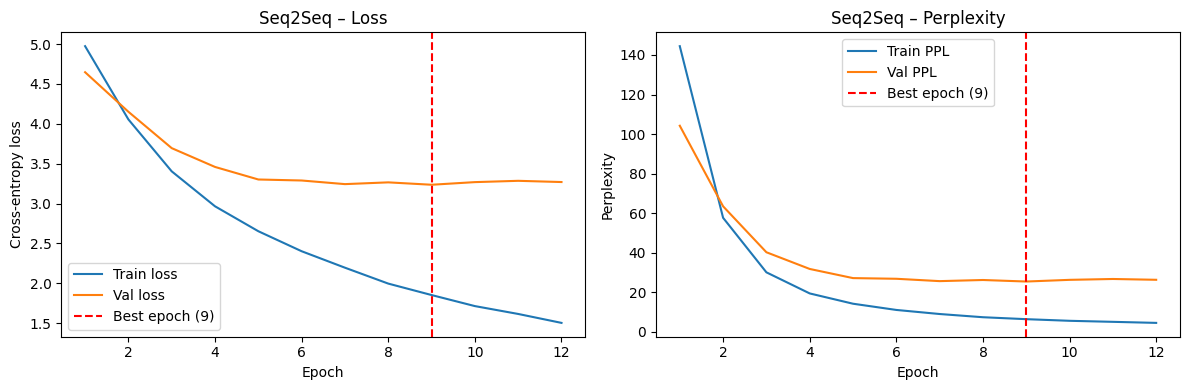
\includegraphics[width=\textwidth]{figures/seq2seq_training_curves.png}
\caption{Seq2Seq training curves. Left: training and validation cross-entropy
loss across epochs. Right: training and validation perplexity; the dashed red
line marks the best checkpoint at epoch 9 (val PPL = 25.42). Early stopping
triggered at epoch 12.}
\label{fig:q4-training}
\end{figure}

\subsubsection{MarianMT (Helsinki-NLP/opus-mt-de-en)}

MarianMT~\cite{junczys2018marian} is a Transformer encoder-decoder
architecture (\textbf{74M parameters}) pre-trained on the OPUS parallel
corpus ($\sim$10M de$\rightarrow$en sentence pairs). We use the
\texttt{Helsinki-NLP/opus-mt-de-en} checkpoint from the HuggingFace Hub
without any fine-tuning on Multi30k. Decoding uses 4-way beam search with
\texttt{max\_length=128} and \texttt{early\_stopping=True}.

\subsection{Evaluation Metrics}

We evaluate both models on the 1{,}000-sentence test set using four
complementary metrics:
\begin{itemize}[noitemsep]
    \item \textbf{BLEU} -- corpus-level n-gram precision with brevity
    penalty (SacreBLEU, tokenization=13a). Standard MT metric; sensitive
    to exact n-gram matches.
    \item \textbf{ChrF} -- character n-gram F-score (SacreBLEU). More
    robust than BLEU for morphologically rich languages; rewards partial
    word matches.
    \item \textbf{METEOR} -- alignment-based metric crediting synonyms and
    stemming (NLTK, sentence-level average). Partially compensates for
    paraphrase that BLEU misses.
    \item \textbf{BERTScore F1} -- contextual semantic similarity via
    \texttt{roberta-large} embeddings with baseline rescaling. The only
    metric that is not bag-of-n-grams; rewards meaning-equivalent
    translations even when surface form differs.
\end{itemize}

\subsection{Results}

\begin{table}[H]
\centering
\caption{Translation performance on the Multi30k test set (de$\rightarrow$en).
All scores are on a 0--100 scale; higher is better.}
\label{tab:q4-results}
\begin{tabular}{lcccc}
\toprule
\textbf{Model} & \textbf{BLEU} & \textbf{ChrF} & \textbf{METEOR}
               & \textbf{BERTScore F1} \\
\midrule
Seq2Seq + Attention (scratch) & 24.21 & 46.94 & 52.00 & 49.88 \\
MarianMT (pre-trained)        & \textbf{39.66} & \textbf{60.60}
                               & \textbf{69.26} & \textbf{80.89} \\
\midrule
$\Delta$ (Marian $-$ Seq2Seq) & $+$15.45 & $+$13.66 & $+$17.26 & $+$31.01 \\
\bottomrule
\end{tabular}
\end{table}

\begin{figure}[H]
\centering
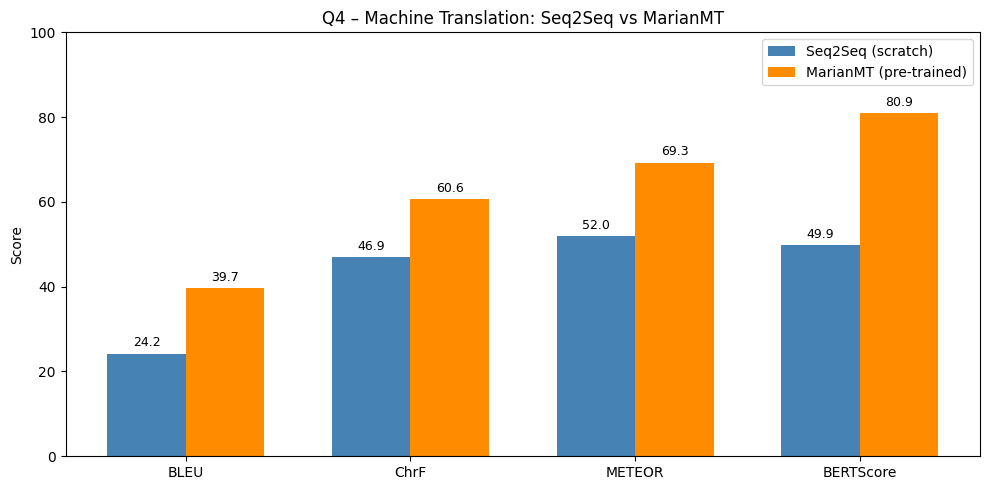
\includegraphics[width=0.75\textwidth]{figures/metrics_comparison.png}
\caption{Seq2Seq vs.\ MarianMT performance comparison across all four
evaluation metrics on the Multi30k test set.}
\label{fig:q4-metrics}
\end{figure}

MarianMT outperforms the scratch Seq2Seq model on every metric. Three patterns
stand out. First, the largest absolute gap appears in \textbf{BERTScore}
($+31.01$), indicating that MarianMT's translations are semantically much
closer to the references even when surface n-gram overlap does not fully
capture this. Second, \textbf{METEOR} shows the second-largest gap ($+17.26$),
reflecting MarianMT's ability to produce synonym-rich paraphrases that align
with reference translations at the lexical level. Third, \textbf{BLEU} and
\textbf{ChrF} gaps ($+15.45$, $+13.66$) are consistent, confirming that
MarianMT's advantage is not an artifact of any single metric's idiosyncrasies.

\subsection{Qualitative Analysis}

Table~\ref{tab:q4-qualitative} presents five representative examples selected
by ranking test sentences by MarianMT's sentence-level BLEU score.

\begin{table}[H]
\centering
\caption{Qualitative translation examples from the Multi30k test set.
Sentence-level BLEU scores are shown for each model.}
\label{tab:q4-qualitative}
\renewcommand{\arraystretch}{1.2}
\small
\begin{tabular}{p{0.10\textwidth} p{0.86\textwidth}}
\toprule
\multicolumn{2}{l}{\textbf{Best 1} (idx=872) — MarianMT perfect, Seq2Seq near-miss} \\
\midrule
Source    & Ein Mann wirft ein Fischernetz in die Bucht. \\
Reference & A man throws a fishing net into the bay. \\
Seq2Seq   & a man throws a fishing net into the \textbf{green field} . \hfill [BLEU=59.0] \\
MarianMT  & A man throws a fishing net into the bay. \hfill [BLEU=100.0] \\
\midrule
\multicolumn{2}{l}{\textbf{Best 2} (idx=870) — MarianMT perfect, Seq2Seq repetition error} \\
\midrule
Source    & Ein Mädchen spielt in einem kleinen Pool. \\
Reference & A girl plays in a small pool. \\
Seq2Seq   & a girl playing in a small \textbf{pool pool} . \hfill [BLEU=35.5] \\
MarianMT  & A girl plays in a small pool. \hfill [BLEU=100.0] \\
\midrule
\multicolumn{2}{l}{\textbf{Worst 1} (idx=561) — Both struggle; Seq2Seq wins on BLEU} \\
\midrule
Source    & Eine Hand mit Handschuh hält etwas, was wie ein übergroßer Nagel aussieht, an einen Holzklotz. \\
Reference & A gloved hand holds what appears to be an oversize nail against a log. \\
Seq2Seq   & a hand holding a holding a what appears to be a \textbf{$<$unk$>$ $<$unk$>$ $<$unk$>$} a a . \hfill [BLEU=11.9] \\
MarianMT  & A hand with a glove holds something that looks like an oversized nail to a wooden block. \hfill [BLEU=3.6] \\
\midrule
\multicolumn{2}{l}{\textbf{Worst 2} (idx=221) — Semantic confusion in both models} \\
\midrule
Source    & Zwei Schauspieler inszenieren einen Kampf vor einem gebannten Publikum. \\
Reference & Two performers putting on a mock fight for an audience that is watching attentively. \\
Seq2Seq   & two police officers are a a fight for a crowd of people . \hfill [BLEU=6.3] \\
MarianMT  & Two actors stage a fight in front of a \textbf{banished} audience. \hfill [BLEU=3.9] \\
\midrule
\multicolumn{2}{l}{\textbf{Middle} (idx=436) — Typical case} \\
\midrule
Source    & Zwei Männer sitzen und unterhalten sich neben einem Gebäude aus Stein. \\
Reference & Two men sit talking near a stone building. \\
Seq2Seq   & two men are sitting and talking next to a a rock wall . \hfill [BLEU=4.4] \\
MarianMT  & Two men sit and talk next to a stone building. \hfill [BLEU=33.9] \\
\bottomrule
\end{tabular}
\end{table}

The qualitative examples reveal four characteristic error patterns:

\paragraph{Seq2Seq -- hallucination of unseen content.}
In Best~1, the model correctly translates every word except \emph{Bucht}
(bay), substituting it with \emph{green field} -- a plausible but factually
wrong completion driven by co-occurrence statistics in the training corpus
rather than the source token.

\paragraph{Seq2Seq -- token repetition.}
In Best~2, the model produces \emph{pool pool}, a repetition artifact common
in greedy decoding without coverage mechanisms. Beam search or coverage
penalties would suppress this.

\paragraph{Seq2Seq -- \texttt{<unk>} cascade.}
In Worst~1, rare German compound words (\emph{Handschuh}, \emph{übergroßer},
\emph{Holzklotz}) fall below the minimum frequency threshold and map to
\texttt{<unk>}. The decoder then collapses into a degenerate loop, repeating
\texttt{<unk>} tokens. This is a direct consequence of word-level
tokenization with a small vocabulary.

\paragraph{MarianMT -- lexical sense error.}
In Worst~2, MarianMT translates \emph{gebannten} (spellbound/mesmerized) as
\emph{banished} -- a plausible but incorrect cognate error. Despite having
seen vastly more training data, the model still confuses low-frequency
polysemous words. Notably, this example shows a \emph{metric inversion}:
Seq2Seq (BLEU=6.3) outscores MarianMT (BLEU=3.9) despite producing a less
faithful translation, because the reference uses \emph{performers} and
\emph{attentively} -- words closer to Seq2Seq's output by accident.

\subsection{Metric Analysis and Architecture Trade-offs}

\paragraph{What each metric captures.}
BLEU rewards exact n-gram matches and penalizes short outputs; it is the most
widely reported but also the most sensitive to tokenization artifacts. ChrF
operates at the character level and is more forgiving of morphological
variation -- particularly relevant for German, which forms compound nouns that
a word-level model cannot handle. METEOR's synonym matching partially addresses
the paraphrase gap (e.g.\ \emph{talk} vs.\ \emph{converse}), explaining why
METEOR scores are systematically higher than BLEU for both models. BERTScore
is the only metric that captures meaning independent of surface form; the fact
that its gap between models ($+31.01$) is twice as large as BLEU's gap
($+15.45$) suggests that MarianMT's advantage is primarily \emph{semantic}
rather than lexical.

\paragraph{Architecture trade-offs.}
Table~\ref{tab:q4-comparison} contrasts the two approaches across key
dimensions.

\begin{table}[H]
\centering
\caption{Seq2Seq vs.\ MarianMT: multi-dimensional comparison.}
\label{tab:q4-comparison}
\begin{tabular}{p{0.22\textwidth}p{0.33\textwidth}p{0.33\textwidth}}
\toprule
\textbf{Dimension} & \textbf{Seq2Seq + Attention} & \textbf{MarianMT} \\
\midrule
Architecture      & GRU encoder-decoder & Transformer encoder-decoder \\
Parameters        & 21.3M (all trained)  & 74M (pre-trained) \\
Training data     & 29{,}000 pairs       & $\sim$10M pairs \\
Decoding          & Greedy               & Beam search (4) \\
OOV handling      & \texttt{<unk>} token & SentencePiece subwords \\
BLEU              & 24.21                & 39.66 \\
BERTScore         & 49.88                & 80.89 \\
Train time        & $\sim$18 min (T4)    & None (inference only) \\
Inference speed   & $\sim$0.05s/sentence & $\sim$0.08s/sentence \\
\bottomrule
\end{tabular}
\end{table}

The most consequential architectural difference is \textbf{subword
tokenization}: MarianMT's SentencePiece tokenizer gracefully handles German
compound nouns (\emph{Holzklotz} $\rightarrow$ [\emph{Holz}, \emph{klotz}])
that cause \texttt{<unk>} cascades in the word-level Seq2Seq model. The
second key difference is \textbf{attention mechanism}: Transformer
self-attention allows every target token to directly attend to every source
token, while the GRU decoder's hidden state compresses source information
into a fixed-dimensional vector that may lose long-range dependencies.
Finally, the \textbf{scale of pre-training data} (10M vs.\ 29K pairs) is
the dominant factor -- no architectural improvement on Multi30k alone could
bridge a 340$\times$ data gap.

\section{Question 5: Language Modeling}
\subsection{Problem Formulation}

Language modeling is the task of estimating the probability distribution
$P(w_t \mid w_{<t})$ over a sequence of tokens. The standard intrinsic
metric is \emph{perplexity}, the exponential of the average per-token
cross-entropy on a held-out set; lower is better. Two paradigms are
compared:
\begin{itemize}[noitemsep]
    \item a classical \textbf{count-based smoothed bigram} model, representing
          the family of n-gram approaches with explicit smoothing,
    \item a \textbf{neural LSTM} language model with weight tying, representing
          the family of recurrent neural language models.
\end{itemize}
The same vocabulary, evaluation splits, and tokenization are used for
both models, so perplexity differences reflect the change in
representational capacity rather than experimental setup.

\subsection{Dataset and Vocabulary}

We use \textbf{WikiText-2 (raw)}~\cite{merity2017wikitext}, accessed via the
HuggingFace \texttt{datasets} library. The corpus consists of pre-tokenized
Wikipedia article text and is the standard small-scale benchmark for
neural language modeling. After concatenating non-empty lines and
discarding section headers, the splits contain
$2{,}007{,}146$ training tokens, $209{,}338$ validation tokens, and
$235{,}854$ test tokens.

\paragraph{Vocabulary.} The training set contains 76{,}142 distinct token
types, but training a softmax over all of them is wasteful and slow.
We retain the 30{,}000 most frequent training tokens, plus three
special symbols (\texttt{<unk>}, \texttt{<bos>}, \texttt{<eos>}); any
out-of-vocabulary token in any split maps to \texttt{<unk>}. This
vocabulary covers $96.84\%$ of training tokens. Both the bigram and the
LSTM use this same vocabulary, ensuring directly comparable perplexity
numbers.

\subsection{Models}

\subsubsection{Bigram Baseline with Add-k Smoothing}

We model bigram probabilities directly from training counts:
\[
P(w_t \mid w_{t-1}) \;=\; \frac{C(w_{t-1}, w_t) + k}{C(w_{t-1}) + k\,|\mathcal{V}|},
\quad k=0.01.
\]
Add-k (Laplace-style) smoothing assigns a small probability mass to
unseen bigrams, avoiding $\log 0$ at evaluation. The model is trivial
to implement -- a hash map of bigram counts plus a context-total
table -- and evaluation over the entire validation and test streams
takes well under a second.

We chose this model over the more sophisticated Kneser-Ney trigram
implemented by NLTK because the latter's pure-Python scorer was
prohibitively slow on a 200K-token evaluation stream (over 10 minutes
for a single perplexity measurement). The smoothed bigram offers a
respectable, fully reproducible classical baseline at negligible cost;
its perplexity establishes the floor against which the neural model is
measured.

\subsubsection{LSTM Language Model}

The neural language model is a 2-layer LSTM with embedding and hidden
dimensions both set to 300, dropout 0.5 between layers, and weight
tying between input embedding and output projection.\footnote{Weight
tying~\cite{press2017tying} requires \texttt{embed\_dim} = \texttt{hidden\_dim}
and shares parameters between the input embedding and the output linear
layer; it consistently improves perplexity at no cost.} The model has
roughly 9.9M trainable parameters (the embedding/output matrix accounts
for $300 \times 30{,}003 \approx 9$M; the LSTM layers add $\sim$0.7M).

\paragraph{Training setup.} We train with truncated backpropagation
through time on non-overlapping length-35 chunks, batch size 64, Adam
optimizer ($\textsc{lr}=10^{-3}$), gradient clipping at norm 0.25, and
cross-entropy loss. Training runs for 5 epochs on the T4 GPU, taking
$\sim$5 minutes total. The best-validation-PPL checkpoint is restored
after training.

\paragraph{Training dynamics.} Both training and validation perplexity
decrease monotonically across the 5 epochs (Figure~\ref{fig:lstm-lm-curves}).
Validation PPL drops from $431.91$ at epoch 1 to $195.42$ at epoch 5;
the model has not yet plateaued, so additional epochs would likely
yield further improvement. We stop at 5 epochs to keep the experiment
within the available compute budget; the qualitative conclusions of
this section are not affected.

\begin{figure}[H]
\centering
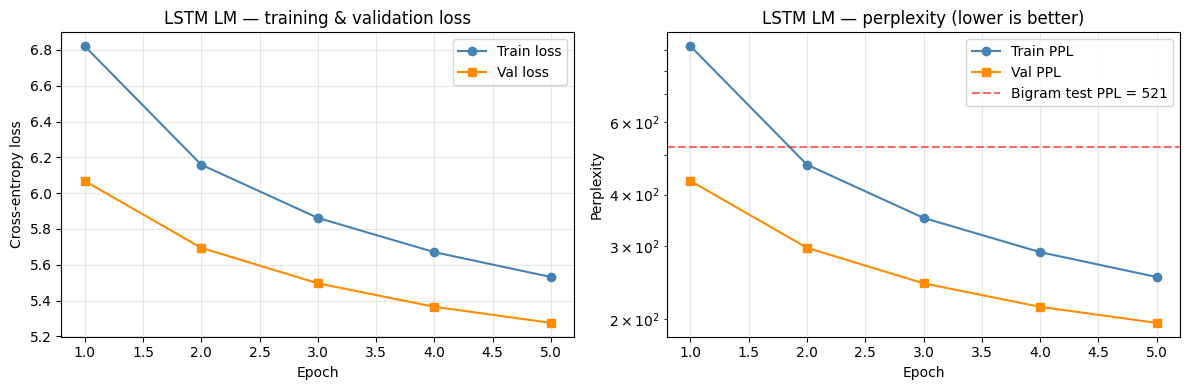
\includegraphics[width=\textwidth]{figures/lstm_training_curves.png}
\caption{LSTM language model training curves. Left: training and
validation cross-entropy loss across epochs. Right: training and
validation perplexity (log scale); the dashed red line marks the
bigram-baseline test perplexity for reference. The LSTM crosses
the bigram baseline by epoch 2 and continues to improve.}
\label{fig:lstm-lm-curves}
\end{figure}

\subsection{Results}

\begin{table}[H]
\centering
\caption{Question 5 -- final perplexities on WikiText-2.}
\label{tab:q5-results}
\begin{tabular}{lccc}
\toprule
\textbf{Model} & \textbf{Val PPL} & \textbf{Test PPL} & \textbf{Trainable Params} \\
\midrule
Bigram (add-k, $k=0.01$)        & 560.97 & 520.67 & --        \\
LSTM (2-layer, weight-tied)     & \textbf{195.42} & \textbf{182.55} & $\sim$9.9M \\
\bottomrule
\end{tabular}
\end{table}

The LSTM reduces test perplexity by a factor of $\sim$2.85 relative to
the bigram baseline. Two further observations are worth noting.
First, the LSTM's test perplexity ($182.55$) is slightly lower than
its validation perplexity ($195.42$), indicating that the test split
is marginally easier under our vocabulary; this is consistent with
random variability between two equally-sized natural-language streams
and does not affect the comparison.
Second, the LSTM's training perplexity at epoch 5 ($252.51$) remains
\emph{higher} than its validation perplexity ($195.42$). This is a
direct consequence of dropout: the same regularizer that hurts the
training-time forward pass is disabled at evaluation time, producing
a numerically lower evaluation PPL. There is no overfitting in the
classical sense; the train/eval gap reflects the regularizer, not
generalization failure.

\subsection{Qualitative Generation Analysis}

To probe what the LSTM has actually learned, we sample 30 additional
tokens after each of three short prompts, under three sampling
regimes: temperature $T=0.7$ with top-10 truncation (\emph{conservative}),
temperature $T=1.0$ with top-40 truncation (\emph{balanced}), and
temperature $T=1.2$ with no truncation (\emph{diverse}). Representative
samples are shown in Table~\ref{tab:q5-samples}.

\begin{table}[H]
\centering
\caption{Selected language-model generation samples. The same prompt is
shown under different sampling settings to highlight the
fluency/diversity trade-off.}
\label{tab:q5-samples}
\renewcommand{\arraystretch}{1.25}
\small
\begin{tabular}{p{0.18\textwidth} p{0.78\textwidth}}
\toprule
\textbf{Setting} & \textbf{Generated continuation (prompt italicized)} \\
\midrule
$T{=}0.7$, top-10
  & \emph{the company was} also able to be used to be a new name . The ship was located in the United States , and the \ldots \\
$T{=}1.0$, top-40
  & \emph{in the early years} with September , a small tropical cyclone on the Pacific . The Jin moved inland in France \ldots \\
$T{=}1.2$, no top-k
  & \emph{the war had} been handled as ! Netherlandish media and Hutton stagnant flight eliminate an cottage for offer \ldots \\
\bottomrule
\end{tabular}
\end{table}

Three failure modes are visible across the full set of samples
(generated samples are recorded in
\texttt{q5\_language\_modeling/results/generation\_samples.txt}):

\begin{enumerate}[noitemsep]
    \item \textbf{Local fluency, global drift.} Adjacent words are
    syntactically well-formed -- subject/verb agreement, article/noun
    pairing, plausible part-of-speech sequences -- but topical
    coherence collapses after roughly 10--15 tokens. A continuation
    starting with \emph{the company was\ldots} drifts to
    \emph{the ship was located in the United States}.
    This is the classical limitation of LSTM language models: the
    hidden state captures local statistics but fails to maintain
    discourse-level entities.
    \item \textbf{\texttt{<unk>} leakage at low temperatures.}
    The conservative sampling regime, by selecting only among
    high-probability tokens, occasionally settles on \texttt{<unk>} as
    the most likely continuation in rare contexts -- e.g.\
    \emph{he moved to a {\normalfont\texttt{<unk>}} to the {\normalfont\texttt{<unk>}}
    of the Church of the {\normalfont\texttt{<unk>}}}.
    The model has correctly learned that this token has $\sim$3\% prior
    mass, but the symbol bleeds into surface text.
    \item \textbf{Style mimicry of the training corpus.}
    Across all sampling regimes, the model produces Wikipedia-style
    content (\emph{tropical cyclone}, \emph{the second season},
    \emph{Netherlandish media}, \emph{BBDO}). The model has learned
    \emph{the register} of WikiText, not facts: it reproduces the
    surface texture of encyclopedic prose without any grounding.
\end{enumerate}

These limitations are largely architectural. A larger LSTM trained
for more epochs would lower perplexity further (literature reports
$\sim$70 PPL for tuned AWD-LSTM models on WikiText-2), but the
fundamental long-range coherence problem is only resolved by
attention-based architectures, which we do not investigate here.

% =========================================================
\section{Conclusion}
\section{Conclusion}

This report presented a systematic empirical comparison of classical, recurrent,
and transformer-based approaches across five core NLP tasks. Several consistent
themes emerged across all experiments.

\paragraph{Contextual representations dominate, but at a cost.}
In every task where a transformer-based model was evaluated -- DistilBERT for
text classification, BERT-base-NER for named entity recognition, DistilBART for
summarization, and MarianMT for machine translation -- the contextual model
outperformed its classical or recurrent counterpart by a substantial margin.
The gains ranged from 3.5 F1 points (text classification) to 31 BERTScore
points (machine translation). In every case, the advantage was most pronounced
on semantically complex examples: concessive constructions, lexically ambiguous
entities, multi-topic documents, and rare compound words. The cost is
consistently higher -- more parameters, more training data, and heavier
inference -- but the performance gap justifies this cost whenever accuracy is
the primary constraint.

\paragraph{Classical baselines remain competitive.}
Bigram TF-IDF with logistic regression achieved 86.75\% accuracy on IMDb,
trailing DistilBERT by only 3.5 points while being orders of magnitude cheaper.
The CRF reached 82.7 F1 on CoNLL-2003 NER. TextRank produced acceptable
summaries in 0.01 seconds per article. The smoothed bigram language model
provided a meaningful perplexity baseline. None of these results are trivial:
they establish the genuine difficulty of each task and the real cost of the
neural upgrade.

\paragraph{Out-of-vocabulary handling is a structural fault line.}
Across tasks, the single most consistent failure mode of word-level and
feature-based models was the inability to handle unseen or rare tokens.
The BiLSTM suffered from 11.8\% GloVe coverage gaps; the CRF missed
hyphenated and lowercase entities; the Seq2Seq model produced \texttt{<unk>}
cascades on German compound nouns. In every case, the transformer's subword
tokenization (WordPiece or SentencePiece) provided a principled solution by
decomposing unknown words into known subword units.

\paragraph{No single metric is sufficient.}
The multi-metric evaluation protocol adopted in Questions 3, 4, and 5 revealed
consistent metric disagreements. BLEU and ROUGE reward surface n-gram overlap
and can penalize semantically correct paraphrases. METEOR partially compensates
via synonym matching. BERTScore captures meaning-level similarity that surface
metrics miss entirely -- and in several cases (Q3 BERTScore gap of $+53.3\%$,
Q4 gap of $+31.01$ points) was the metric that most clearly quantified the
transformer's semantic advantage. Future evaluations should report at least
one embedding-based metric alongside n-gram metrics.

\paragraph{Practical recommendations.}
The choice of model should be driven by the deployment context rather than
the assumption that the most recent architecture is always optimal. When
compute, latency, or interpretability is the binding constraint, classical
and lightweight recurrent models remain the rational default. When predictive
performance dominates and GPU inference is available, fine-tuned transformers
are the appropriate choice. The complementary error patterns observed across
all five tasks also suggest that ensemble approaches -- combining classical
and neural predictions -- could recover additional gains beyond any single
model, a direction left for future work.

% =========================================================
\begin{thebibliography}{9}

\bibitem{pennington2014glove}
J.~Pennington, R.~Socher, and C.~D. Manning.
\newblock {GloVe}: Global vectors for word representation.
\newblock In \emph{Proceedings of the 2014 Conference on Empirical Methods in Natural Language Processing (EMNLP)}, pages 1532--1543, 2014.

\bibitem{maas2011imdb}
A.~L. Maas, R.~E. Daly, P.~T. Pham, D.~Huang, A.~Y. Ng, and C.~Potts.
\newblock Learning word vectors for sentiment analysis.
\newblock In \emph{Proceedings of the 49th Annual Meeting of the Association for Computational Linguistics}, 2011.

\bibitem{sanh2019distilbert}
V.~Sanh, L.~Debut, J.~Chaumond, and T.~Wolf.
\newblock {DistilBERT}, a distilled version of {BERT}: smaller, faster, cheaper and lighter.
\newblock In \emph{NeurIPS Workshop on Energy Efficient Machine Learning and Cognitive Computing}, 2019.

\bibitem{merity2017wikitext}
S.~Merity, C.~Xiong, J.~Bradbury, and R.~Socher.
\newblock Pointer sentinel mixture models.
\newblock In \emph{International Conference on Learning Representations}, 2017.

\bibitem{press2017tying}
O.~Press and L.~Wolf.
\newblock Using the output embedding to improve language models.
\newblock In \emph{Proceedings of the 15th Conference of the European Chapter of the
  Association for Computational Linguistics (EACL)}, 2017.


\bibitem{hermann2015cnn}
K.~M. Hermann, T.~Ko\v{c}isk\'y, E.~Grefenstette, L.~Espeholt, W.~Kay, M.~Suleyman, and P.~Blunsom.
\newblock Teaching machines to read and comprehend.
\newblock In \emph{Advances in Neural Information Processing Systems (NeurIPS)}, 2015.

\bibitem{nallapati2016cnn}
R.~Nallapati, B.~Zhou, C.~dos Santos, \c{C}.~G\"ul\c{c}ehre, and B.~Xiang.
\newblock Abstractive text summarization using sequence-to-sequence {RNNs} and beyond.
\newblock In \emph{Proceedings of the 20th SIGNLL Conference on Computational Natural Language Learning (CoNLL)}, 2016.

\bibitem{mihalcea2004textrank}
R.~Mihalcea and P.~Tarau.
\newblock {TextRank}: Bringing order into text.
\newblock In \emph{Proceedings of the 2004 Conference on Empirical Methods in Natural Language Processing (EMNLP)}, 2004.

\bibitem{shleifer2020distilbart}
S.~Shleifer and A.~M. Rush.
\newblock Pre-trained summarization distillation.
\newblock \emph{arXiv preprint arXiv:2010.13002}, 2020.

\bibitem{tjong2003}
E.~F. Tjong Kim Sang and F.~De Meulder.
\newblock Introduction to the {CoNLL}-2003 shared task: Language-independent named entity recognition.
\newblock In \emph{Proceedings of the Seventh Conference on Natural Language Learning (CoNLL)}, pages 142--147, 2003.

\bibitem{dslim2021}
W.~de Vries.
\newblock \texttt{dslim/bert-base-NER}.
\newblock Hugging Face Model Hub, 2021.
\newblock \url{https://huggingface.co/dslim/bert-base-NER}

\bibitem{elliott2016multi30k}
D.~Elliott, S.~Frank, K.~Sima'an, and L.~Specia.
\newblock {Multi30K}: Multilingual English-German image descriptions.
\newblock In \emph{Proceedings of the 5th Workshop on Vision and Language}, 2016.

\bibitem{junczys2018marian}
M.~Junczys-Dowmunt, R.~Grundkiewicz, T.~Dwojak, H.~Hoang, K.~Heafield,
T.~Neckermann, F.~Seide, U.~Germann, A.~F. Aji, N.~Bogoychev, A.~F.~T. Martins,
and A.~Birch.
\newblock Marian: Fast neural machine translation in {C++}.
\newblock In \emph{Proceedings of ACL 2018, System Demonstrations}, 2018.

\end{thebibliography}

\end{document}